\subsubsection{\idx{Pitagora}}

\zadatak Odredi $x$ sa slike.
$$
\slika{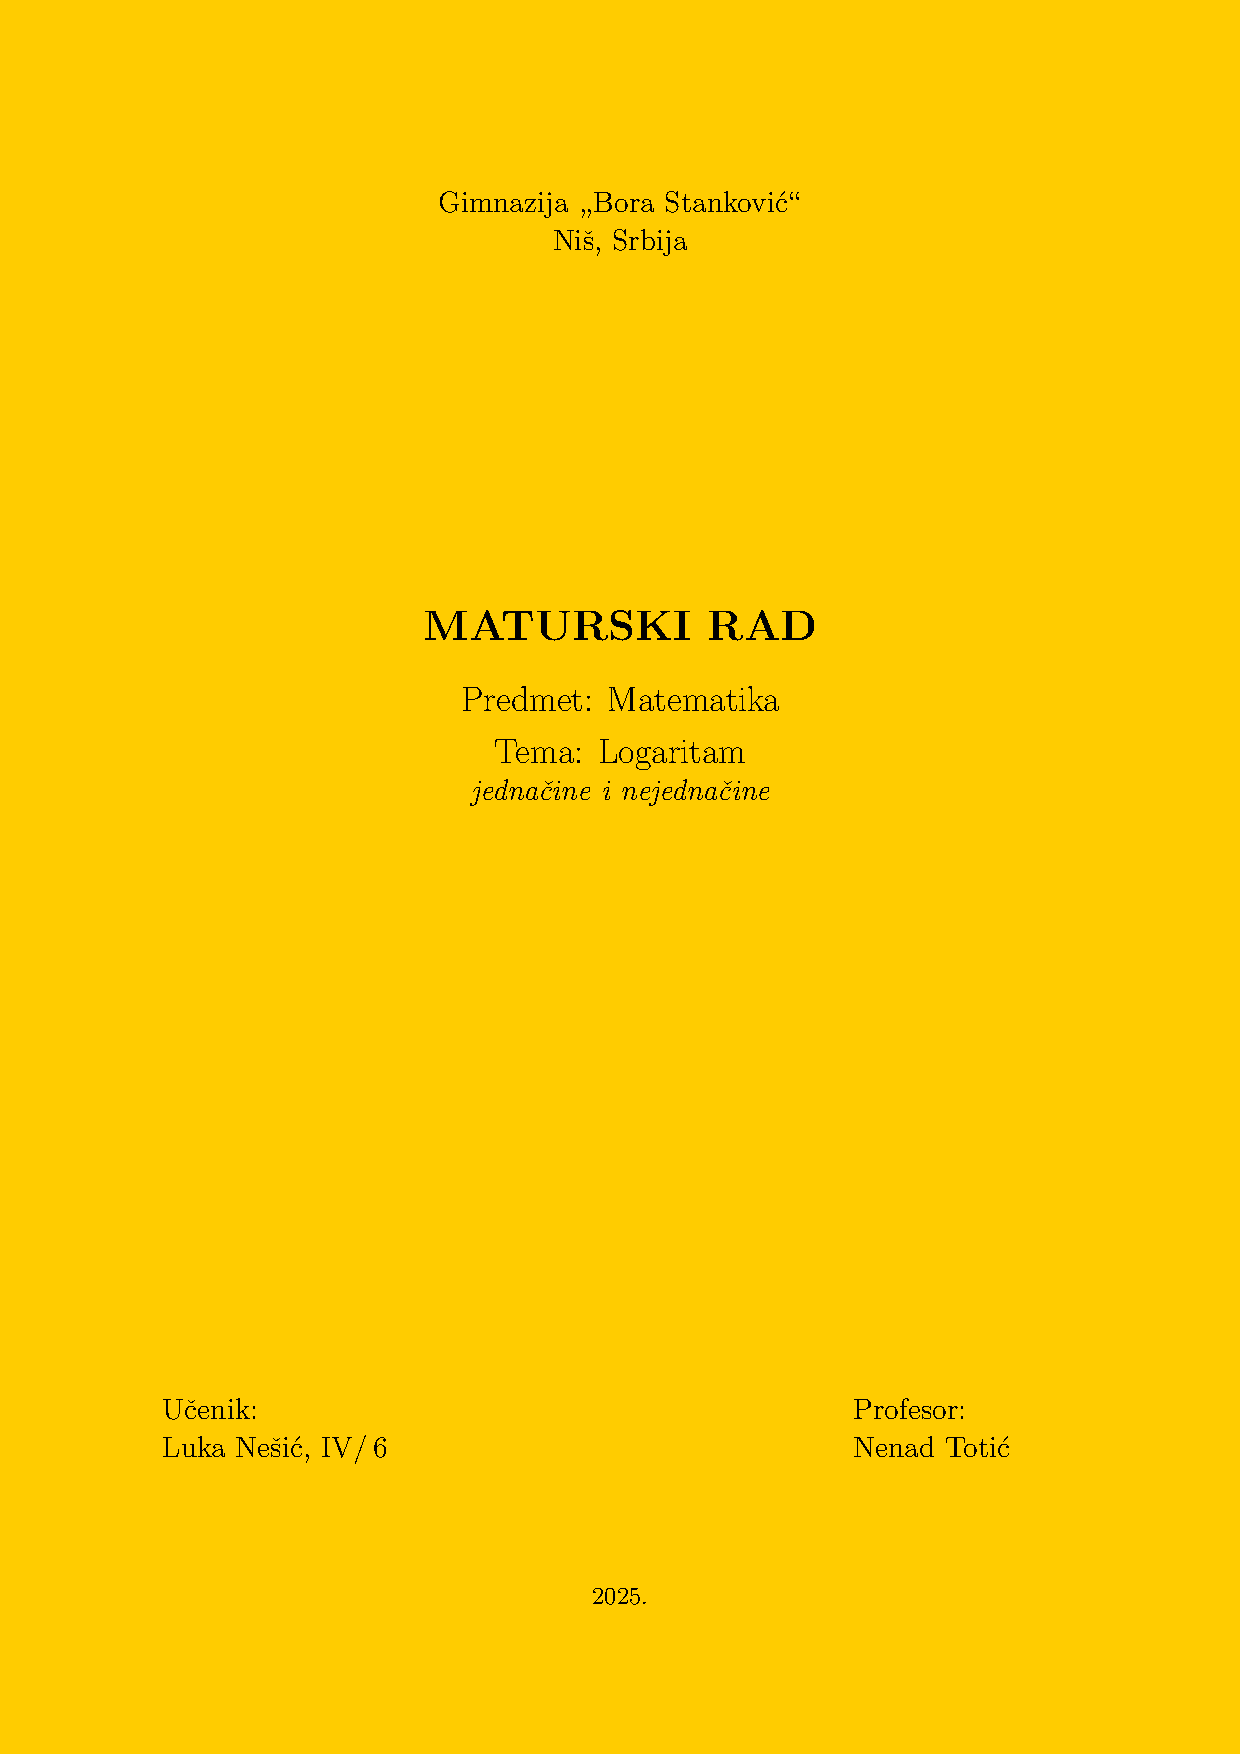
\includegraphics[]{log.5}}{Pravougli \idx{trougao}\index{pravougli trougao} $\triangle ABC$.}
$$
(Zadatak sa {\sl Tik-Toka\index{TikTok@Tik-Tok}}.)

\resenje
Kako je $a=\ln x$, $b=a+\ln2$ i $c=a+\ln3$, iz {\sl Pitagorine teoreme\/}\index{Pitagorina teorema} 
$a^2 + b^2 = c^2$, sledi da je
\begin{align*}
    a^2+(a+\ln2)^2 &= (a+\ln3)^2.
\intertext{Kada izvr{\sv}imo smenu $u=\ln2$ i $v=\ln3$, dobijamo}
    a^2 + a^2 + 2au + u^2 &= a^2 +2av +v^2,
\end{align*}
gde posle sre{\dj}iva{\nj}a, dobijamo kvadratnu jedna{\cv}inu\index{kvadratna jedna{\cv}ina}
$$
a^2+2(u-v)a+(u^2-v^2)=0,
$$
koja ima dva re{\sv}e{\nj}a
\begin{align*}
a_{1,2}&= (v - u) \pm \sqrt{2v(v-u)},
\intertext{ali nas zanima samo pozitivno. Kako je $v-u=\ln3-\ln2=\ln(3/2)$, dobijamo}
a&=\ln\left(\frac32\right) + \sqrt{2\ln 3\ln\left(\frac32\right)}.
\end{align*}
Odavde je
$$
x=\e^a=\ram{\frac32\, \e^{\sqrt{2\ln 3\ln(3/2)}}}
\approx 3\.85488,
$$
a stranice trougla su pribli{\zv}no
$$
a\approx 1\.34934, \quad b\approx 2\.04249, \quad c\approx 2\.44795.
$$
(Na slici su stranice skalirane sa $3\um{cm}$.)
